% Needed and Layout
\documentclass[a4paper,11pt]{article}
\usepackage[utf8]{inputenc} % utf8 encoding
\usepackage{amsfonts}
\usepackage[T1]{fontenc} % use for allowing < and > in cleartext
\usepackage[margin=2.5cm]{geometry}

% Lists
\usepackage{verbatim}   % useful for program listings
\usepackage{enumitem}
\usepackage[ampersand]{easylist}

% Creating more compact lists
\let\olditemize\itemize
\renewcommand{\itemize}{
    \olditemize
    \setlength{\itemsep}{1pt}
    \setlength{\parskip}{0pt}
    \setlength{\parsep}{0pt}
}


% Creating my own inline code font
\newcommand{\textcode}[1]{
    \texttt{\colorbox{gray!10}{{#1}}}
}


% Math
\usepackage{mathtools}   % need for subequations

% Graphics
\usepackage{graphicx}   % need for figures
\usepackage{color}      % use if color is used in text 
\usepackage{xcolor}     % use for text background color
\usepackage{tikz}
\usetikzlibrary{arrows}
\usepackage{float}

% Other
\usepackage{url}
\usepackage{todonotes}
\usepackage{pdfpages}
\usepackage{subcaption}
\usepackage{latexsym}
\usepackage{fixltx2e}    % use for textsubscript
\usepackage[titletoc,title]{appendix}
\usepackage[framemethod=tikz]{mdframed}
\usepackage[titletoc,title]{appendix}
\usepackage{epstopdf}
\bibliographystyle{plain}

% Code listing
\usepackage{listings} % For inserting code from file (I think)
\usepackage{algorithm}
\usepackage{algpseudocode}
\renewcommand{\algorithmicforall}{\textbf{for each}}
\makeatletter
\def\BState{\State\hskip-\ALG@thistlm}
\makeatother

\DeclareCaptionFormat{algor}{%
  \hrulefill\par\offinterlineskip\vskip1pt%
    \textbf{#1#2}#3\offinterlineskip\hrulefill}
\DeclareCaptionStyle{algori}{singlelinecheck=off,format=algor,labelsep=space}
\captionsetup[algorithm]{style=algori}

% URLs ? maybe
\usepackage[hypcap=false]{caption}
\usepackage{hyperref}


% I wonder what this is
\definecolor{codegreen}{rgb}{0,0.6,0}
\definecolor{codegray}{rgb}{0.5,0.5,0.5}
\definecolor{codepurple}{rgb}{0.58,0,0.82}
\definecolor{backcolour}{rgb}{1.0,1.0,1.0}
\lstdefinestyle{mystyle}{
  backgroundcolor=\color{backcolour},   commentstyle=\color{codegreen},
  keywordstyle=\color{magenta},
  numberstyle=\tiny\color{codegray},
  stringstyle=\color{codepurple},
  basicstyle=\footnotesize,
  breakatwhitespace=false,         
  breaklines=true,                 
  captionpos=b,                    
  keepspaces=true,                 
  numbers=left,                    
  numbersep=5pt,                  
  showspaces=false,                
  showstringspaces=false,
  showtabs=false,                  
  tabsize=2
}
\lstset{style=mystyle}

\begin{document}

% Configuration
\setlength{\parindent}{0cm}
\setlength{\unitlength}{1mm}

% Front Page
\date{September 1st 2015\\ IT University of Copenhagen}
\title{A Quantitative Analysis of Bugs in Linux}
\author{Elvis Flesborg\\
\texttt{efle@itu.dk}}
\clearpage\maketitle
\thispagestyle{empty}
\newpage

%%%%%%%%%%%%%%%%%%%%%%%%%%%%%%%%%%%%%%%%%%%%%%%%%%%%%%%%%%%%%%%%%%%%%%%%%%%%%%%%
%                           TABLE OF CONTENTS
%%%%%%%%%%%%%%%%%%%%%%%%%%%%%%%%%%%%%%%%%%%%%%%%%%%%%%%%%%%%%%%%%%%%%%%%%%%%%%%%
\tableofcontents
\thispagestyle{empty}



\newpage

\setcounter{page}{1}

\section{Abstract}
\emph{---Leave blank until the end---}

\section{Introduction}
\emph{---Leave blank until the end---}


% TODO
\begin{itemize}
    \item \underline{\textbf{TODO}}
        \item Explain about representative samples
\end{itemize}


%%%%%%%%%%%%%%%%%%%%%%%%%%%%%%%%%%%%%%%%%%%%%%%%%%%%%%%%%%%%%%%%%%%%%%%%%%%%%%%%
%                           BACKGROUND
%%%%%%%%%%%%%%%%%%%%%%%%%%%%%%%%%%%%%%%%%%%%%%%%%%%%%%%%%%%%%%%%%%%%%%%%%%%%%%%%
\newpage
\section{Background}

\subsection{The Linux Kernel}

Many software products are configurable in some way. This creates the 
possibility of tailoring the software to suit different needs. For example 
different kinds of hardware, or different funtionalities.

The Linux Kernel is probably the one open source software product with more 
than 19M lines of code 
\footnote{http://www.phoronix.com/misc/linuxstat-june-2015/files.html}, 
which has the highest configurability\footnote{source}. It is also said that a 
software product has a large amount of \emph{Variability}\footnote{Is it 
called that?} \\


This represents that the software system has many options that can be turned 
on or off, or can be given a specific value. These options will here be called 
\emph{features}.

The Linux kernel has around 11,000 features in the feature 
model\footnote{\$grep bla bla}. This means that Linux is highly configurable, 
and possibly the reason for Linux to have such great scalability (it can be 
used in everything from small embedded devices to supercomputers) 
\footnote{find source}. \\


This high variability rate makes maintaining the code somewhat harder to 
grasp, and this makes the code base more error prone. So what you get in 
scalability you pay for in hardness of maintaining the code. \footnote{Refer 
to Jean's project or something}.


\subsubsection{The linux-next tree}

\begin{center}
    \emph{
        Comment from the linux-next page or something
    }
\end{center}

The Linux Kernel development cycle has approximately 2$\frac{3}{4}$ months 
from one stable release to the next stable 
release\footnote{http://phb-crystal-ball.org/}. In the meantime, \emph{RC} 
releases, also called \emph{prepatch} releases, are released once in a while. 
Mainly for kernel developers to test for new features.  \\


Then there is the \emph{linux-next} tree. It is a \emph{git} tree, which 
merges over 200 other \emph{git} trees\footnote{See <src>/Next/Trees}, which 
all are based on the \emph{mainline} tree. The \emph{linux-next} tree is 
merging these other trees every day and the merge conflicts are handled. 
Therefore the \emph{linux-next} tree always contain the newest commits. 

This tree will get some bugs fixed sooner than if everyone contributed to the 
mainline and tested on that. Comparing to a stable version, one would suspect 
the \emph{linux-next} tree to have more bugs, since it has not been tested, 
and it is the newest code available, which means more bugs have been inserted. 
\\


For this thesis project, both the \emph{linux-next} tree and the latest stable 
version is used. As time of writing, the latest stable version is \emph{4.1.1}.

\footnote{http://neuling.org/linux-next-size.html}

\footnote{http://news.gmane.org/gmane.linux.kernel.next - the linux-next 
mailing list archive}

\footnote{http://kisskb.ellerman.id.au/kisskb/matrix/ - this is some kind of 
build robot results page.}

\footnote{
http://git.kernel.org/cgit/linux/kernel/git/next/linux-next.git/tree/Next/Trees
?id=HEAD - here are all the git trees that are merged in linux-next}


% TODO
\begin{itemize}
    \item \underline{\textbf{TODO}}
    \item Find out how to find the exact number of possible configurations. It 
        is in some article, I got by Andrzej. Plus maybe SharpSAT.
    \item Explain how to find the number of features by grepping.
    \item Talk about subsystems
    \item Maybe talk about the percentage of code in every subsystems. What is 
        Linux Kernel made of?
    \item talk about who contributes to the kernel. (intel, novell). Both in 
        code and money?
\end{itemize}


\subsection{Kconfig}

The Kconfig language is the language of the feature model in Linux (also used 
for other projects like busybox, vim, etc...). In this chapter, I will shortly 
explain the ups and downs of the Kconfig language. \\


The different data types are pretty much the same as with a normal programming 
language. Although with the exception of \emph{tristate}, which can be $[y, n, 
m]$. The list is \emph{boolean}, \emph{tristate}, \emph{string}, \emph{hex}, 
and \emph{integer}.

Every feature must have a data type, and a description. It can then have the 
following other options:

\begin{itemize}
    \item Default values
    \item Help text
    \item Features that this feature depends on
    \item Features that depends on this feature
\end{itemize}

Also there is the \emph{choice} option, where only one of multiple features 
can be enabled. \\


This can all be visualized in an \emph{Abstract Syntax Tree}, or a dependency 
tree. I will show a tiny example because the whole feature model of Linux 
Kernel is far too big.


% TODO
\begin{itemize}
    \item \underline{\textbf{TODO}}
    \item Explain how kconfig is shattered over many files.
    \item It creates a `.config` file.
    \item How many are of each data type?
    \item Explain the Kconfig language a bit
    \item Show a dependency tree
    \item Examples of constraints in the language
    \item Reference to Thorsten's projects
    \item Refer to the /Documentation/kbuild/kconfig-language.txt
\end{itemize}

\subsection{randconfig}

The Linux Kernel comes with different ways of creating your own configuration 
file. There is a question based one (\emph{config}), and some menu based ones 
(\emph{menuconfig}, \emph{xconfig}, \emph{nconfig}, \emph{gconfig}), but also 
some that will never prompt the user for anything, but create some automated 
config (\emph{allyesconfig}, \emph{allnoconfig}, \emph{defconfig}, and 
\emph{randconfig}).

That last one \emph{randconfig} is interesting, as it will go through the 
Kconfig feature model files, and pick random values for all of the features. 
This should be perfect for the goal for this project. Although time will tell 
that it is indeed biased, and will not create configurations that are of 
representative character. 

See figure for a toy example of this.


\begin{center}
    \emph{-- figure --}
\end{center}


This shows that it is highly likely that \emph{randconfig} will have a strong 
bias towards features that are in the top of the dependency tree comparing to 
the features that are deeper down in the dependency tree. 

To actually create a representative sample of the configuration space was 
proven to be harder than was initially thought. A couple of methods were 
thought out to make the configuration creation more representative. \\


One idea was to alter the code for \emph{randconfig}, to make it know how deep 
the dependency tree was, and make it bias the coin flipping process correctly. 
For example if landing a \emph{yes} would yield a total of 99 possible other 
features, and landing a \emph{no} did not yield any other features, then the 
coin should have a 1\% of landing a \emph{no} and a 99 \% chance of landing a 
\emph{yes}. \\


Another idea was to take all the spread out Kconfig files, and concatenate 
them all into one big text file, which would then be modified. If the order of 
the features were randomized, then the coins would not be flipped in the same 
order every time, and this could have an effect on the dependent features. \\

The third idea was to manually generate a configuration file, and then check - 
somehow - if the config file was valid, and then use it if it was valid. By 
not looking at dependencies, but only considering \emph{choice} options and 
enabling \emph{mandatory features}, a configuration file was created by 
randomly flipping a coin per each feature.

This seemed doable until after generating 100,000 configurations, not one 
valid configuration was found. It seems like many of the $2^{11,000}$ 
configurations are invalid.


% TODO
\begin{itemize}
    \item \underline{\textbf{TODO}}
    \item Show some code of randconfig not doing it representatively
    \item Show a graph with a toy example
    \item show the 33-33 vs 25-25-50 example
\end{itemize}


\subsection{gcc bug types}

When a configuration has been created, the Linux Kernel is compiled using 
that configuration file. This is done mainly by \emph{GNU 
gcc}\footnote{http://gcc.gnu.org/}, which then outputs warning and error 
messages. If there is an error, the compilation will also stop immediately.

These output messages hold the information that will be used in this project. 
In a warning, there is information about a possible coding mistake that might 
break the code. There are about 30 different warning types \footnote{source}. 
Some of these are not so interesting as others for this project.\\


In this project, all the toy examples are made up, and not taken from the 
actual Linux Kernel. \\


Generally there will be distinguished between four different types of output. 
These are \emph{relevant errors}, \emph{irrelevant errors}, \emph{relevant 
warnings}, and \emph{irrelevant warnings}. 


\paragraph{The relevant errors} are errors that will occur on all machines 
when a certain configuration is being built. 

A difficult task is to figure out what exactly caused the error. 
\footnote{Give a list of possible errors... I found that site}


\paragraph{The irrelevant errors} 
are a result of the building system not having some specific dependencies 
installed. 

For instance, there is a feature in the feature model that is called 
\textbf{CONFIG\_KERNEL\_LZO}, which dictates that the kernel should be 
compressed by the \emph{lzop} library instead of the default \emph{gzip} 
compression library.

When a randomly configurated kernel has the \textbf{CONFIG\_KERNEL\_LZOP} 
enabled - which would happen approximately every 6th random configuration - 
then to build the kernel the \emph{lzop} library will have to be installed on 
the build system. If it was not, then the compilation would crash with the 
same error. \\ 


There exist many other examples like this in the \emph{Linux Kernel} where an 
uninstalled program will result in an unbuilt kernel. These \emph{irrelevant 
errors} would have to be minimized, since they are not actual kernel errors, 
but local errors. \footnote{Give list of all the features I have disabled}


\paragraph{The relevant warnings}
are warnings that may cause an error at some point. The \emph{uninitialized 
variable} warning is such a warning. If a variable is uninitialized, and ends 
up being called, it may cause an error, and stop the compilation.

\lstinputlisting[language=C]{code/uninitializedvar.c}

This will return the warning \textcode{'a' is used uninitialized in this 
function [-Wuninitialized]} and the output, when the program is run, will
be \textcode{0Hello world}.

\paragraph{The irrelevant warnings}
These are mainly warnings that represent dead code. Warnings like \emph{unused 
function}, \emph{unused variable}, \emph{unused label}, and \emph{unused 
value}, will all end up as dead code, which is bad for fitting a kernel 
on some hardware with limited space. Apart from that it is nothing else than 
code pollution. \\

\lstinputlisting[language=C, firstline=3]{code/unusedvar.c}

This will return the warning \textcode{unused variable 'a' [-Wunused-variable]}


\lstinputlisting[language=C, firstline=3]{code/unusedfunc.c}

This will return the warning \textcode{'func' defined but not used 
[-Wunused-function]}. Notice, that the function will have to be static for the 
warning to show.


% TODO
\begin{itemize}
    \item \underline{\textbf{TODO}}
    \item Give real examples of unused function, and uninitialed... bla
    \item Give unreal examples of ditto
\end{itemize}


%%%%%%%%%%%%%%%%%%%%%%%%%%%%%%%%%%%%%%%%%%%%%%%%%%%%%%%%%%%%%%%%%%%%%%%%%%%%%%%%
%                           METHODOLOGY
%%%%%%%%%%%%%%%%%%%%%%%%%%%%%%%%%%%%%%%%%%%%%%%%%%%%%%%%%%%%%%%%%%%%%%%%%%%%%%%%
\newpage
\section{Methodology}

The objective is to make a quantitative analysis of errors and warnings in the 
Linux Kernel based on as many random configurations as are possible to generate 
within the time span of this project.

There will be generated random configurations, and these will be used to 
compile two Linux Kernels. One stable Linux Kernel, and one from the 
linux-next repository.  \\


\subsection{Research Questions}

RQ1: Will the unstable linux-next repository generate more errors than the 
stable kernel. \\


RQ2: Can it be seen what warnings are mostly generated. An ordered list of the 
different warnings types.  \\


RQ3: Can it be seen in what subsystems most errors occur. And in the 
largest subsystems, in what subsubsystem? \\


RQ4: What percentage of the possible configurations for the Kernel are valid. \\


RQ5: Are there any specific features, that when enabled, will produce more 
warnings than others. \\




\subsection{Collecting data}

Every time a randomly configured compilation is running, \emph{gcc} will 
output warning and error messages in the \emph{standard error} output. This 
output is then scraped through to categorize it.

An output line will contain a \emph{bug type}, a \emph{filename}, \emph{line 
number}, and a \emph{message} describing the warning in english.


The collection of data has mainly been done on a computer at the IT University 
of Copenhagen. It has 32 cores and 128 GB of RAM, and the mean time to compile 
a kernel and upload the data was around 1 minute and 35 seconds. A fairly 
regular laptop with 4 cores and 8 GB of RAM does that in just over 8 minutes 
on average.

\begin{itemize}
    \item Grepping the stderr
    \item Categorizing the warnings/Errors
    \item About the collection machine
    \item About the database setup
\end{itemize}




%%%%%%%%%%%%%%%%%%%%%%%%%%%%%%%%%%%%%%%%%%%%%%%%%%%%%%%%%%%%%%%%%%%%%%%%%%%%%%%%
%                                 DATA
%%%%%%%%%%%%%%%%%%%%%%%%%%%%%%%%%%%%%%%%%%%%%%%%%%%%%%%%%%%%%%%%%%%%%%%%%%%%%%%%
\newpage
\section{Data}

\begin{itemize}
    \item Example of data structure
    \item Graph of tables
\end{itemize}




%%%%%%%%%%%%%%%%%%%%%%%%%%%%%%%%%%%%%%%%%%%%%%%%%%%%%%%%%%%%%%%%%%%%%%%%%%%%%%%%
%                               RESULTS
%%%%%%%%%%%%%%%%%%%%%%%%%%%%%%%%%%%%%%%%%%%%%%%%%%%%%%%%%%%%%%%%%%%%%%%%%%%%%%%%
\newpage
\section{Results}

\subsection{Analyzing the data}

\subsection{Number of valid configurations}

\subsection{Observations}




%%%%%%%%%%%%%%%%%%%%%%%%%%%%%%%%%%%%%%%%%%%%%%%%%%%%%%%%%%%%%%%%%%%%%%%%%%%%%%%%
%                           THREATS TO VALIDITY
%%%%%%%%%%%%%%%%%%%%%%%%%%%%%%%%%%%%%%%%%%%%%%%%%%%%%%%%%%%%%%%%%%%%%%%%%%%%%%%%
\newpage
\section{Threats to Validity}

\begin{itemize}
    \item Only run on x86 architecture
    \item randconfig bias
    \item firmware blobs
    \item 
\end{itemize}

\subsection{Generate'n'Filter}

\begin{itemize}
    \item Uniform distribution
    \item Too low percentage
    \item Get a lower bound on the percentage
    \item sharpSAT?
\end{itemize}

\subsection{elvisconfig}

\begin{itemize}
    \item Maybe the permutation script can be used elsewhere (Thorsten seemed 
        interested)
\end{itemize}

\subsection{RandomSAT}





%%%%%%%%%%%%%%%%%%%%%%%%%%%%%%%%%%%%%%%%%%%%%%%%%%%%%%%%%%%%%%%%%%%%%%%%%%%%%%%%
%                           RELATED WORK
%%%%%%%%%%%%%%%%%%%%%%%%%%%%%%%%%%%%%%%%%%%%%%%%%%%%%%%%%%%%%%%%%%%%%%%%%%%%%%%%
\newpage
\section{Related Work}

\begin{itemize}
    \item 42 bugs
    \item Variability in ...
    \item Paper from Iago
    \item Fengguang Wu and Intel
\end{itemize}



\newpage
\section{Conclusion}
\emph{--- Leave empty until the end---}




\newpage
\bibliography{bibliography}

\end{document}

% Example of Bibliography
\newpage
\bibliography{bibliography}

% Example of Appendix
\begin{appendices}
\section{Code}
\lstinputlisting[language=Python]{../temp.py}
\end{appendices}

% Example of a drawing
\begin{figure}[H]
    \begin{center}
        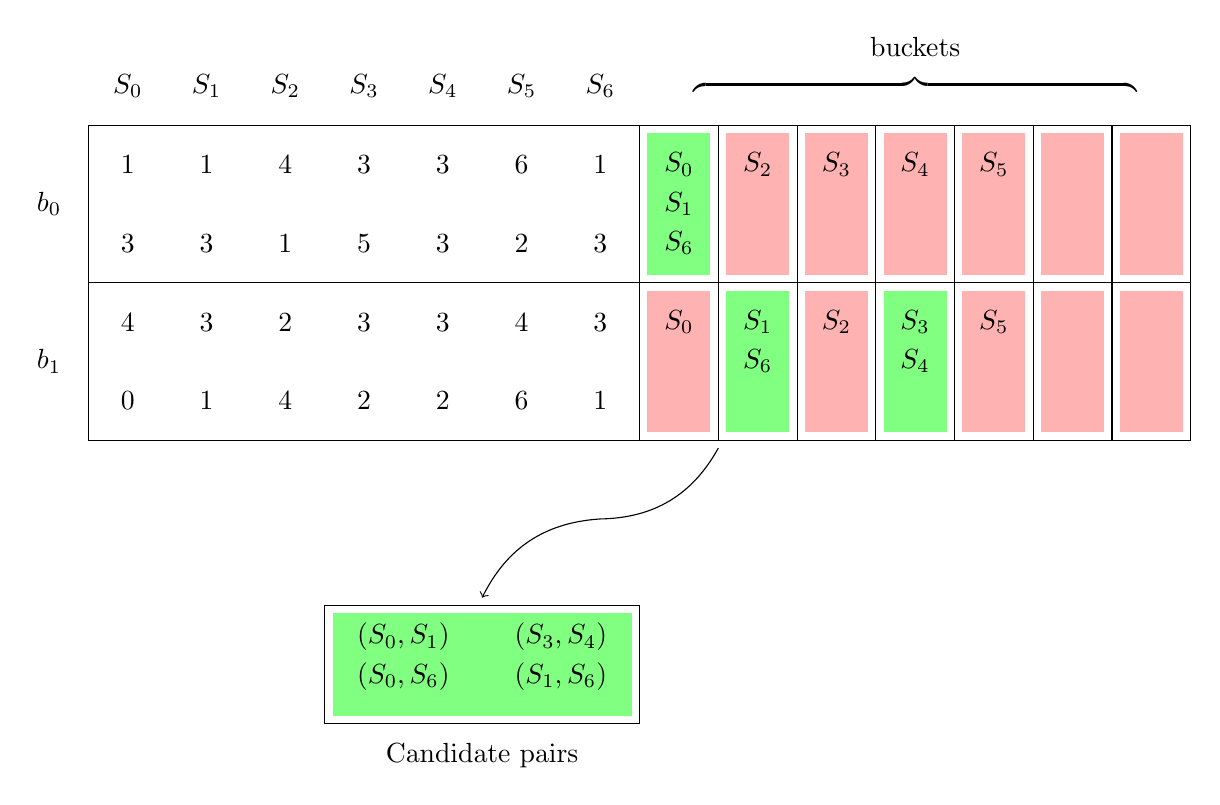
\begin{tikzpicture}
            \draw rectangle (14,4);
            \draw rectangle (7,2);
            \draw (0,2) rectangle (7,2);
            \draw (7,0) rectangle (8,4);

            \foreach \x in {0,...,6} \draw (\x+7, 0) rectangle (\x+7+1, 2);
            \foreach \x in {0,...,6} \draw (\x+7, 2) rectangle (\x+7+1, 4);
            \foreach \x in {0,...,6} \draw (\x+.5, 4.5) node {$S_\x$};

            \draw (-.5,3) node {$b_0$};
            \draw (-.5,1) node {$b_1$};

            % The overbrace
            \draw (10.5, 4.5) node {$\overbrace{\qquad\qquad\qquad\qquad\qquad\qquad\qquad\qquad}$};
            \draw (10.5,5.0) node {buckets};

            % Signature matrix (left part)
            \draw (0.5,3.5) node {1};
            \draw (0.5,2.5) node {3};
            \draw (0.5,1.5) node {4};
            \draw (0.5,0.5) node {0};

            \draw (1.5,3.5) node {1};
            \draw (1.5,2.5) node {3};
            \draw (1.5,1.5) node {3};
            \draw (1.5,0.5) node {1};

            \draw (2.5,3.5) node {4};
            \draw (2.5,2.5) node {1};
            \draw (2.5,1.5) node {2};
            \draw (2.5,0.5) node {4};

            \draw (3.5,3.5) node {3};
            \draw (3.5,2.5) node {5};
            \draw (3.5,1.5) node {3};
            \draw (3.5,0.5) node {2};

            \draw (4.5,3.5) node {3};
            \draw (4.5,2.5) node {3};
            \draw (4.5,1.5) node {3};
            \draw (4.5,0.5) node {2};

            \draw (5.5,3.5) node {6};
            \draw (5.5,2.5) node {2};
            \draw (5.5,1.5) node {4};
            \draw (5.5,0.5) node {6};

            \draw (6.5,3.5) node {1};
            \draw (6.5,2.5) node {3};
            \draw (6.5,1.5) node {3};
            \draw (6.5,0.5) node {1};

            % Fill all with red (in right part)
            \foreach \x in {0,...,6} \path[fill=red!30] (7.1+\x,0.1) rectangle (7.9+\x,1.9);
            \foreach \x in {0,...,6} \path[fill=red!30] (7.1+\x,2.1) rectangle (7.9+\x,3.9);

            % Fill the right ones with green
            \path[fill=green!50] (7.1,2.1) rectangle (7.9,3.9);
            \path[fill=green!50] (8.1,0.1) rectangle (8.9,1.9);
            \path[fill=green!50] (10.1,0.1) rectangle (10.9,1.9);

            % Names
            \draw (7.5,3.5) node {$S_0$};
            \draw (7.5,3.0) node {$S_1$};
            \draw (7.5,2.5) node {$S_6$};
            \draw (8.5,3.5) node {$S_2$};
            \draw (9.5,3.5) node {$S_3$};
            \draw (10.5,3.5) node {$S_4$};
            \draw (11.5,3.5) node {$S_5$};

            \draw (7.5,1.5) node {$S_0$};
            \draw (8.5,1.5) node {$S_1$};
            \draw (8.5,1.0) node {$S_6$};
            \draw (9.5,1.5) node {$S_2$};
            \draw (10.5,1.5) node {$S_3$};
            \draw (10.5,1.0) node {$S_4$};
            \draw (11.5,1.5) node {$S_5$};


            % Arrows
            \path[-] (8,-.1) edge [bend left] (6.5,-1);
            \path[->] (6.5,-1) edge [bend right] (5,-2);

            % Candidate squares
            \path[fill=green!50] (3.1, -3.5) rectangle (6.9, -2.2);
            \draw (3,-3.6) rectangle (7,-2.1);

            % Candidate signatures
            \draw (4,-2.5) node {$(S_0, S_1)$};
            \draw (4,-3.0) node {$(S_0, S_6)$};
            \draw (6,-3.0) node {$(S_1, S_6)$};
            \draw (6,-2.5) node {$(S_3, S_4)$};

            \draw (5,-4.0) node {Candidate pairs};
            

        \end{tikzpicture}
    \caption{LSH buckets and bands}
    \label{fig:lsh_buckets}
    \end{center}
\end{figure}


% Example of algorithm
\begin{center}   
    \captionof{algorithm}{Locality Sensitive Hashing algorithm}\label{alg:lsh}
    \begin{algorithmic}
    
    \BState \textbf{Calculate signature matrix as in algorithm \ref{alg:minhashing}}\\

    \State $SIG\gets \text{signature matrix}$
    \State $S\gets \text{number of signatures}$
    \State $bucket\_list\gets \text{empty list}$
    \State $B\gets \text{number of bands}$\\

    \BState \emph{Fill the buckets}
    \For{$b_i$ in $i = 0 \ldots B-1$}
        \State $h_i \gets \text{empty dictionary}$
        \State $bucket\_list.append(h_i)$
        \For{$SIG_j[b_i]$ in $j = 0 \ldots S-1$}
            \State $key \gets SIG_j[b_i]$
            \If{$key$ in $h_i$}
                \State $bucket \gets h_i[key]$
            \Else
                \State $bucket \gets \text{empty list}$
            \EndIf
            \State $bucket.append(j)$
        \EndFor
    \EndFor\\

    \State $candidate\_pairs \gets \text{empty set}$
    \ForAll{$h_i$ in $bucket\_list$}
        \ForAll{$key$ in $h_i$}
            \State $bucket \gets h_i[key]$
            \If{$bucket.length > 1$}
                \For{$pair$ in $bucket$}
                    \State $candidate\_pairs.add(pair)$ 
                \EndFor
            \EndIf
        \EndFor        
    \EndFor\\

    \BState \textbf{Calculate similarities from signature matrix as in algorithm \ref{alg:minhashing}, for the candidate pairs.}

    \end{algorithmic}
\end{center}


% Example of a gnuplot input
\begin{figure}[H]
    \begin{center}
        \input{plots/scurve.tex}
        \caption{S-curve - $f(s) = 1 - (1 - s^r)^b$ ; $k = 1000$}
        \label{fig:scurve}
    \end{center}
\end{figure}


% Example of a table
\begin{figure}[H]
    \begin{center}
        \begin{tabular}{c|c|c}
              & Actual & LSH \\
            \hline
            1 & 1.0 & 1.0 \\
            2 & 1.0  & 1.0 \\
            3 & 0.667 & 0.702 \\
            4 & 0.667 & 0.695 \\
            5 & 0.667 & 0.689 \\
            6 & 0.667 & 0.684 \\
            7 & 0.667 & 0.681 \\
            8 & 0.667 & 0.681 \\
            9 & 0.667 & 0.677 \\
            10 & 0.667 & 0.673 
        \end{tabular}
        \caption{Correctness of LSH}
        \label{tab:lsh-correctness}
    \end{center}
\end{figure}


% Example of equation
\begin{equation}
    \frac{B(64;R,r_1,r_2)}{B(1;R,r_1,r_2} \Rightarrow \frac{64 R}{R + 1 - r_1}
    \label{eq:improvementratio}
\end{equation}


% Example of graphic
\begin{figure}[H]
    \begin{center}
        \includegraphics{plots/bbit/bbit.eps}
        \caption{b-Bit storage improvement}
        \label{fig:bbit}
    \end{center}
\end{figure}
